\section{Background}
\label{sec:background}

\subsection{Brief introduction to SystemJ syntax, semantics and model of
  computation}
\label{sec:brief-intr-syst}

\begin{table}[tb]
\centering
\caption{SystemJ kernel statements and their meaning}
\begin{minipage}{8cm}
  \begin{small}
   \begin{tabular}{|c|p{80pt}|}
     \hline                                                                                     
     \textbf{Kernel Statements} & \textbf{Meaning}\\                                            
     \hline                                                                                     
     \hline                                                                                     
     [\textbf{\texttt{input}}] [\textbf{\texttt{output}}]
     [\textbf{\texttt{type}}] \textbf{\texttt{signal}} S & declare signal S\\                                      
     \hline                                                                                     
     \textbf{\texttt{emit}} S [(value)] & broadcast signal S\\                                                    
     \hline                                                                                     
     \textbf{\texttt{present}} (S) \{p\} else \{q\}& do p if S is present, else do q\\                            
     \hline                                                                                     
     \textbf{\texttt{abort}} (S) \{p\} & preempt program p if S is present\\                                      
     \hline                                                                                     
     \textbf{\texttt{suspend}} (S)\{p\} & suspend p if S is present\\                                             
     \hline                                                                                     
     \textbf{\texttt{trap}} (T)\{p\ldots \textbf{\texttt{exit}} T\ldots\} & preempt p if exit is executed\\                         
     \hline                                                                                     
     p\textbf{\texttt{$||$}}q & run p and q in lock-step\\                                                        
     \hline                                                                                     
     p$><$q & run p and q asynchronously\\                                                      
     \hline                                                                                     
     \textbf{\texttt{send}} C([value]) & send a value through C, blocking
     send\\                                                 
     \hline                                                                                     
     \textbf{\texttt{receive}} C() & receive a value through C, blocking
     receive\\
     \hline                                                                                     
     \textbf{\texttt{pause}} & finish a tick and communicate
     with environment\\
     \hline                                                                                     
   \end{tabular}
  \end{small}
   % \footnotetext[1]{\scriptsize Uppercase}
 \end{minipage}
 \label{tab:1}
\end{table}

Table~\ref{tab:1} presents the SystemJ kernel statements used to program
the control flow. The data-flow is programmed in Java. A number of
derived statements also exist (e.g., \texttt{sustain}, \texttt{await},
etc) that make programming reactive systems easier. The \textit{Model of
  Computation} (MoC) of a simple SystemJ is shown in Figure~\ref{fig:2}.

\begin{figure*}[bth]
\centering
\begin{SubFloat}{\label{fig:2a}Simple SystemJ program}%...verbatim subfigure
\begin{minipage}[b]{0.3\linewidth}% a minipage to control the width...
\begin{verbatim}
while(true){
 abort(A){
  while(true)
   pause;
  emit O;
  // do java computation
}
\end{verbatim}%
\end{minipage}%
\end{SubFloat}
\hspace{1.5cm}%
\begin{SubFloat}[Black box]{\label{fig:2b}Ticks in SystemJ}%
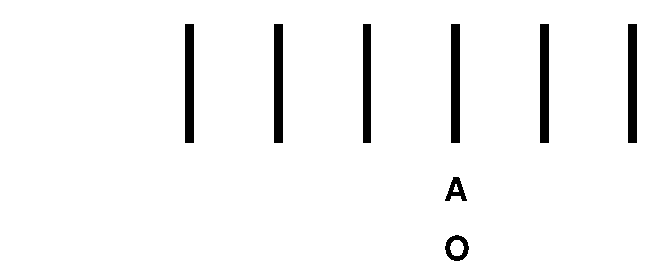
\includegraphics[scale=0.5]{moc}
\end{SubFloat}%
\caption{Simple SystemJ example and corresponding MoC}
\label{fig:2}
\end{figure*}

SystemJ consists of entities called clock-domains (CD)s, each running at
their individual pace. Each CD adheres to the \textit{perfect synchrony}
hypothesis, i.e., all statements execute instantaneously in zero
time. Only the \texttt{pause} statement consumes time, just like in
Esterel~\cite{gber931}. Consider the SystemJ program in
Figure~\ref{fig:2a}, it is waiting for an input signal producing logical
ticks (see Figure~\ref{fig:2b}). Once \texttt{A} is received at tick 4,
output \texttt{O} is emitted to the environment instantaneously.

\subsection{Mapping logical time to physical time}
\label{sec:mapping-logical-time}

The perfect synchrony hypothesis is ideal for programming the
synchronous sub-set of SystemJ. But, the real-world is not that
forgiving, execution of every \textit{micro-step} in the logical zero
time, requires $\delta$ physical time. Time for a complete reaction to
one or more input signal can thus be summarized as $\Delta = \Sigma
(\delta)$. We call $\Delta$ the reaction time. Obviously depending upon
the amount of computation required, $\Delta$ can vary, hence, in order
to satisfy the implicit restriction posed by the synchrony hypothesis --
no input event can be missed, one needs to calculate the \textit{Worst
  Case Reaction Time} (WCRT) and the resultant WCRT needs to be smaller
than the speed of the fastest input event, else the synchrony hypothesis
is violated. A substantial amount of research for calculating the WCRT
of synchronous programs~\cite{proop10,boldt07,wilhelm08} exists. We
refer the reader to any of these research articles, since WCRT analysis
is not the focus of this paper. The opposite of the WCRT is the
\textit{Best Case Reaction Time} (BCRT), we denote the WCRT and BCRT in
Figure~\ref{fig:2b} using \texttt{W} and \texttt{B}, respectively.

We now present two lemmas with proof sketch (due to lack of space) that
we require for the rest of the paper.

\begin{lemma}
  WCRT and BCRT analysis are invariant to values of conditional
  expressions.
\end{lemma}

\begin{proof}
  The physical time ($\delta$) taken by a conditional expression is at
  best affected by the type rather than the value of the
  conditional. Example, comparing the value of 2 floats might take
  longer than comparing the value of 2 integer types on some given
  platform. But, the time taken by the comparison instruction is
  invariant to the value itself.
\end{proof}

\begin{lemma}
  WCRT and BCRT analysis are invariant to channel communication.
\end{lemma}
\begin{proof}
  LATER ....
\end{proof}


%%% Local Variables: 
%%% mode: latex
%%% TeX-master: "paper"
%%% End: 
